\documentclass[letterpaper,12pt,twoside]{uncthesis}

\usepackage{pgfplots}
\usepackage{tikz}
\usepackage{dcolumn}
\usepackage{soul}

\newcommand{\betrfs}{BetrFS\xspace}
\newcommand{\betrfsOne}{BetrFS 0.1\xspace}
\newcommand{\betrfsTwo}{BetrFS 0.2\xspace}
\newcommand{\betrfsThree}{BetrFS 0.3\xspace}
\newcommand{\betrfsFour}{BetrFS 0.4\xspace}
\newcommand{\betrfsFive}{BetrFS 0.5\xspace}
\newcommand{\bet}{B$^{\varepsilon}$-tree\xspace}
\newcommand{\bets}{B$^{\varepsilon}$-trees\xspace}
\newcommand{\btree}{B-tree\xspace}
\newcommand{\btrees}{B-trees\xspace}
\newcommand{\fti}{\textit{ft-index}\xspace}
\newcommand{\Fti}{\textit{Ft-index}\xspace}
\newcommand{\klibc}{\textbf{klibc}\xspace}
\newcommand{\Klibc}{\textbf{Klibc}\xspace}
\newcommand{\mdb}{\texttt{meta\_db}\xspace}
\newcommand{\ddb}{\texttt{data\_db}\xspace}
\newcommand{\spre}{\textit{src\_prefix}\xspace}
\newcommand{\dpre}{\textit{dst\_prefix}\xspace}
\newcommand{\goto}{\texttt{GOTO}\xspace}
\newcommand{\putm}{\texttt{PUT}\xspace}
\newcommand{\delm}{\texttt{DEL}\xspace}
\newcommand{\rdm}{\texttt{RD}\xspace}
\newcommand{\delold}{\textit{del\_old}\xspace}
\newcommand{\bedag}{B$^{\varepsilon}$-DAG\xspace}
\newcommand{\bedags}{B$^{\varepsilon}$-DAGs\xspace}
\newcommand{\xf}{\texttt{xf}\xspace}

\pgfkeys{
    /fs-names/ext4/.initial=ext4,
    /fs-names/btrfs/.initial=Btrfs,
    /fs-names/btrfs-svol/.initial=Btrfs-svol,
    /fs-names/xfs/.initial=XFS,
    /fs-names/zfs/.initial=ZFS,
    /fs-names/nilfs2/.initial=NILFS2,
    /fs-names/betrfs3/.initial=\betrfsThree,
    /fs-names/betrfs3-max/.initial=\betrfsThree with an infinite zone size,
    /fs-names/betrfs4/.initial=\betrfsFour,
    /fs-names/betrfs5/.initial=\betrfsFive,
}

\pgfkeys{
    /fs-colors/ext4/.initial=blue,
    /fs-colors/btrfs/.initial=red,
    /fs-colors/btrfs-svol/.initial=brown,
    /fs-colors/xfs/.initial=green,
    /fs-colors/zfs/.initial=purple,
    /fs-colors/nilfs2/.initial=cyan,
    /fs-colors/betrfs3/.initial=yellow,
    /fs-colors/betrfs3-max/.initial=orange,
    /fs-colors/betrfs4/.initial=orange,
    /fs-colors/betrfs5/.initial=gray,
}

\pgfkeys{
    /fs-marks/ext4/.initial=triangle*,
    /fs-marks/btrfs/.initial=pentagon*,
    /fs-marks/btrfs-svol/.initial=triangle*,
    /fs-marks/xfs/.initial=square*,
    /fs-marks/zfs/.initial=diamond*,
    /fs-marks/nilfs2/.initial=o,
    /fs-marks/betrfs3/.initial=+,
    /fs-marks/betrfs3-max/.initial=oplus,
    /fs-marks/betrfs4/.initial=oplus,
    /fs-marks/betrfs5/.initial=*,
}

\pgfplotsset{
    discard if/.style 2 args={
        x filter/.code={
            \edef\tempa{\thisrow{#1}}
            \edef\tempb{#2}
            \ifx\tempa\tempb
            \def\pgfmathresult{inf}
            \fi
        }
    },
    discard if not/.style 2 args={
        x filter/.code={
            \edef\tempa{\thisrow{#1}}
            \edef\tempb{#2}
            \ifx\tempa\tempb
            \else
            \def\pgfmathresult{inf}
            \fi
        }
    }
}

\newtheorem{invariant}{Invariant}


%%%%%%%%%%%%%%%%%%%%%%%%%%%%%%%%%%%%%%%%%%%%%%%%%%%%%%%%%%%%
% Required thesis information
%%%%%%%%%%%%%%%%%%%%%%%%%%%%%%%%%%%%%%%%%%%%%%%%%%%%%%%%%%%%

% When indicating your degree in the second bracketed space, use the full
% degree name (i.e., Doctor of Philosophy, not Ph.D. or PHD; Master of Public
% Health, not M.P.H. or MPH; Master of Social Work, not M.S.W. or MSW).
\uncdegreename{Doctor of Philosophy}

% List your department, school, or curriculum rather than your subject area or
% specialty discipline in the third bracketed space. You may include your
% subject area or specialty discipline in parentheses (i.e., Department of
% Romance Languages (French); School of Pharmacy (Molecular Pharmaceutics);
% School of Education (School Psychology); or similar official area).
% If you wish to include both your department and school names, list the school
% at the end of the statement (i.e., Department of Pharmacology in the School
% of Medicine).
\uncthesisdepartment{Department of Computer Science}

% Type can be dissertation or thesis
\uncthesistype{dissertation}

% Title
\uncthesistitle{Efficient, Locality-Maintaining Namespace Operations in a Write-Optimized File System}

% Name
\uncthesisauthor{Yang Zhan}

% University Name
\uncthesisuniversity{University of North Carolina at Chapel Hill}

% The year in which your committee approves the completed thesis or
% dissertation. This need not be the year you graduate.
\uncthesisyear{2019}

% Thesis advisor. Appears on the abstract page.
\uncthesisadvisor{Donald E. Porter}

% Thesis committee. Appears on the title page.  Do not include titles such as
% Professor, Doctor, Dr., PhD, or any identifiers such as “chair” or “advisor”
% before or after any names.  Put a new line after each name to render
% correctly on title page.
\uncthesiscommittee{Donald E. Porter\\
Leonard McMillan\\
F. Donelson Smith\\
Rob Johnson\\
Ethan L. Miller
}

%%%%%%%%%%%%%%%%%%%%%%%%%%%%%%%%%%%%%%%%%%%%%%%%%%%%%%%%%%%%
% Font selection
%%%%%%%%%%%%%%%%%%%%%%%%%%%%%%%%%%%%%%%%%%%%%%%%%%%%%%%%%%%%
% Font, if using PDFLaTeX
\usepackage{times}
% Font, if using XeLaTeX
%\usepackage{fontspec}
%\setmainfont{Times New Roman}

% Prevent awkward hyphenations.
\hyphenation{Raj-kumar}

\begin{document}
% The following order of the contents is REQUIRED
\pagenumbering{roman}


% 1. Title Page
\newgeometry{left=\uncthesisleftmargin in,top=2in,right=\uncthesisrightmargin in,bottom=1in,nohead}

\begin{titlepage}

\begin{singlespace}
\centering

\currentpdfbookmark{TITLE}{bk:title}

\vspace{1in}
\begin{adjustwidth}{0.5in}{0.5in}
\centering
\MakeUppercase{\uncthesistitle}
\end{adjustwidth}

\nointerlineskip\vspace{1in}

\uncthesisauthor{}

\nointerlineskip\vspace{1in}

\noindent
A \uncthesistype{} submitted to the faculty at the \uncthesisuniversity{} in partial fulfillment of the requirements for the degree of \uncdegreename{} in the \uncthesisdepartment{}.

\nointerlineskip\vspace{1in}

Chapel Hill\\
\uncthesisyear{}
%\the\year

\end{singlespace}

% Use the following block if you want the committee members to have exactly a 1in margin to the right.
%\nointerlineskip\vspace{0.83in}
%\setlength\topsep{0pt}
%\begin{flushright}
%{
%\setlength{\tabcolsep}{0pt}
%\begin{tabular}[t]{l}
%Approved by: \\
%\thesismembers
%\end{tabular}
%} % large
%\end{flushright}

% Use the following block if you want the committee members to appear approximately 2/3 the way across the page.
\nointerlineskip\vspace{0.71in}
\begin{flushright}
\begin{minipage}{2.1in}
\setlength{\tabcolsep}{0em}
\begin{tabular}{l}
Approved by: \\
\uncthesiscommittee{}
\end{tabular}
\end{minipage}
\end{flushright}

\end{titlepage}


% 2. Copyright Page (optional)
%\newgeometry{left=\uncthesisleftmargin in,top=8.42in,right=\uncthesisrightmargin in,bottom=1in,nohead}

\begin{center}
\begin{singlespace}
\copyright~\uncthesisyear\\
\uncthesisauthor \\
ALL RIGHTS RESERVED
\end{singlespace}
\end{center}

\clearpage
\newgeometry{left=\uncthesisleftmargin in,top=2in,right=\uncthesisrightmargin in,bottom=1in,nohead}
% Normal pages from here on out; TOC title takes care of 2in requirement.
\restoregeometry


% 3. Abstract
\begin{abstract}

There seems to be a trade-off between good locality and efficient namespace
operations in file systems.
Traditional inode-based file systems have good rename performance, but fail
to maintain locality, especially in the face of file system aging.
On the other hand, full-path-indexed file systems ensure locality, however,
renaming a directory needs to update all related full-paths,
which is usually implemented as an expensive operation.

This dissertation describes a technique that has both good locality and
efficient namespace operations.
In particular, we describe a novel synthesis of write-optimization,
full-path indexing and operations on data structures.
By directly manipulating the data structure, a full-path-indexed file system
can efficiently update related full-paths in a rename.
Moreover, with the technique, a full-path-indexed file system can
clone a directory without traversing the directory.

We implement this technique in \betrfs, a full-path-indexed, write-optimized,
local file system for Linux.
Compared to ext4, the widely used inode-based file system in Linux,
the new version of \betrfs traverses the Linux source directory 9.47x faster,
and renames the same directory 1.09x faster.
Meanwhile, the new version of \betrfs clones a directory faster than
file systems that clone the directory through file clones,
such as Btrfs and XFS.

\end{abstract}


% 4. Dedication, Acknowledgement(s), Preface (each optional)
%\begin{dedication}
A dedication is a message from the author prefixed to a work in tribute to a person, group, or cause. Most dedications are short statements of tribute beginning with \textit{``To \ldots''} such as \textit{``To my family''}.
\end{dedication}

%\begin{acknowledgement}

Acknowledgements are the author's statement of gratitude to and recognition of the people and institutions that helped the author's research and writing.

    \lipsum[5]
\end{acknowledgement}

%\begin{preface}

A preface is a statement of the author's reasons for undertaking the work and other personal comments that are not directly germane to the materials presented in other sections of the thesis or dissertation. These reasons tend to be of a personal nature.

    \lipsum[6]

\end{preface}


% 5. Table of Contents, with page references
\renewcommand{\contentsname}{\hfill\bfseries\normalsize TABLE OF CONTENTS\hfill}
%\renewcommand{\cfttoctitlefont}{\hfill\Large\bfseries}
\renewcommand{\cftaftertoctitle}{\hfill}
\renewcommand{\cftdotsep}{1.5}
\cftsetrmarg{1.0in}

\setlength{\cftbeforetoctitleskip}{56pt}
\setlength{\cftaftertoctitleskip}{18pt}

% format chapter entries like other entries
\renewcommand{\cftchapfont}{\normalfont}
\renewcommand{\cftchappagefont}{\normalfont}
\renewcommand{\cftchapleader}{\cftdotfill{\cftdotsep}}

\setlength{\cftbeforechapskip}{15pt}
\setlength{\cftbeforesecskip}{10pt}
\setlength{\cftbeforesubsecskip}{10pt}
\setlength{\cftbeforesubsubsecskip}{10pt}

\begin{singlespace}
\currentpdfbookmark{TABLE OF CONTENTS}{bk:contents}
\tableofcontents
\end{singlespace}

\clearpage


% 6. List of Tables, with titles and page references (if applicable). And list
% of Figures or Illustrations, with titles and page references (if applicable)
\renewcommand{\listtablename}{LIST OF TABLES}
\phantomsection
\addcontentsline{toc}{chapter}{LIST OF TABLES}

\setlength{\cftbeforelottitleskip}{-14pt}
\setlength{\cftafterlottitleskip}{22pt}
\renewcommand{\cftlottitlefont}{\hfill\normalsize\bfseries}
\renewcommand{\cftafterlottitle}{\hfill}

\setlength{\cftbeforetabskip}{12pt}
\cftsetrmarg{1.0in}

\setlength{\cfttabindent}{0in}

\begin{singlespace}
\listoftables
\end{singlespace}

\clearpage

\renewcommand{\listfigurename}{LIST OF FIGURES}
\phantomsection
\addcontentsline{toc}{chapter}{LIST OF FIGURES}

\setlength{\cftbeforeloftitleskip}{-14pt}
\setlength{\cftafterloftitleskip}{22pt}
\renewcommand{\cftloftitlefont}{\hfill\normalsize\bfseries}
\renewcommand{\cftafterloftitle}{\hfill}

\setlength{\cftbeforefigskip}{12pt}
\cftsetrmarg{1.0in}

\setlength{\cftfigindent}{0in}

\begin{singlespace}
\listoffigures
\end{singlespace}

\clearpage


% 7. List of Abbreviations (if applicable)
%\phantomsection
\addcontentsline{toc}{chapter}{LIST OF ABBREVIATIONS}

\begin{center}
\textbf{LIST OF ABBREVIATIONS}
\vspace{16pt}
\end{center}

% TODO: define new column types to make sure multi-line table cells has single-spacing

\noindent
\begin{tabular}{p{0.8in} p{5in}}
CoS     & Chamber of Secrets\\
DA      & Dumbledore's Army\\
DADA    & Defence Against the Dark Arts\\
DH      & Deathly Hallows \\
FBAWTFT & Fantastic Beasts and Where to Find Them\\
SPEW    & Society for the Protection of Elvish Welfare\\
VWI     & Voldemort War One\\
VWII    & Voldemort War Two\\
\end{tabular}

\clearpage


% 8. List of Symbols (if applicable)
%\phantomsection{}
\addcontentsline{toc}{chapter}{LIST OF SYMBOLS}

\begin{center}
\textbf{LIST OF SYMBOLS}
\vspace{16pt}
\end{center}

\noindent
\begin{tabular}{@{}p{0.8in} l}
$M$ & Number of wands\\
$m$ & Number of wizards\\
$n$ & Number of fantastic beasts\\
\end{tabular}

\clearpage


\pagenumbering{arabic}

%\chapter{Formatting Guide}
\label{chap:formatting_guide}

\section{Margins}

This template follows the UNC graduate school thesis/dissertation formatting guide as rigidly as possible.
This template has uniform margins throughout the entire document:
\begin{itemize}
    \item Left: 1''
    \item Right: 1''
    \item Top: 1''
    \item Bottom: 1''
\end{itemize}

\section{Font}
A TrueType font is recommended/required by the ProQuest dissertation publishing. Recommended fonts and sizes can be found in \autoref{tab:font}.

\begin{table}
    \centering
    \caption{Recommended font type and size}\label{tab:font}
    \begin{tabular}{ll}
        \toprule
        Font name            & Font Size \\ \midrule
        Arial                & 10pt\\
        Century              & 11pt\\
        Courier New          & 10pt\\
        Garamond             & 12pt\\
        Georgia              & 11pt\\
        Lucida Bright        & 10pt\\
        Microsoft Sans Serif & 10pt\\
        Tahoma               & 10pt\\
        Times New Roman      & 12pt\\
        Trebuchet MS         & 10pt\\
        Verdana              & 10pt\\ \bottomrule
    \end{tabular}
\end{table}

If you're using \texttt{pdflatex} to compile this template, include the \texttt{times} package in the preamble.
If you're using \texttt{xelatex} to compile this template, you can use the \texttt{fontspec} package and the \texttt{setmainfont} command to choose your favorite font.
This template by default uses 12pt Times New Roman.

\section{Spacing and Indentation}

The template takes care of spacing and indentation:
\begin{itemize}
    \item Text appears in a single column on each page and is double-spaced throughout the document.
    \item New paragraphs are indicated by a consistent tab indentation throughout the entire document.
    \item The document text is left-justified.
    \item For blocked quotations, indent the entire text of the quotation consistently from the left margin.
\end{itemize}

\lipsum[6]
\begin{quote}
    This is an example showing the indentation of block quoted text.
    \lipsum[8]
\end{quote}
\lipsum[7]

\section{Pagination}
This template takes care of pagination.

Pagination and margin are also well maintained for landscape pages.
\begin{landscape}
    \lipsum[9] Let's also see how does footnote works in landscape pages~\footnote{We have a footnote in landscape environment}.
\end{landscape}

\section{Footnotes and Endnotes}
Footnotes\footnote{\lipsum[10]} and endnotes\footnote{\lipsum[11]} obey the
formatting guide. However, using both of them confuses the note numbering.
Given the discrepancy between the official format guide\endnote{\lipsum[12]}
and the official sample pages\endnote{\lipsum[14]}, the correct order for
endnotes and appendixes are unclear.  Thus, using only footnote is recommended.

\section{Tables and Figures}
Tables, figures, and illustrations vary widely by discipline. Therefore, formatting of these
components is largely at the discretion of the author.

List of figures and list of tables are well taken care of by \LaTeX{} and this
template.  If an entry in LOT/LOF takes up more than one line, break up the
entry about three-fourths of the way across the page and place the rest of the
text on a second line, single-spacing the two lines.

One nice trick is the short caption option for the
\texttt{\textbackslash{}caption{}} command.  It allows the LOT/LOF only include
the short caption but not the full caption.
\begin{figure}
    \centering
    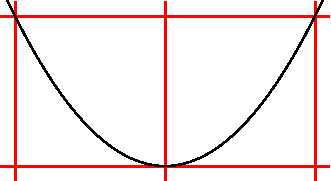
\includegraphics[width=0.5\textwidth]{figures/demo.pdf}
    \caption{A very long caption that does not make much sense but only tests the line-breaking and line-spacing in LOT/LOF.}
\end{figure}

\begin{figure}
    \centering
    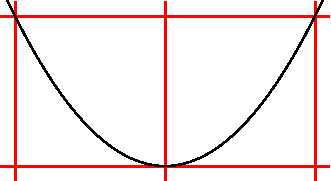
\includegraphics[width=0.5\textwidth]{figures/demo.pdf}
    \caption[Short Caption]{A very long caption that does not make much sense but only tests the line-breaking and line-spacing in LOT/LOF.}
\end{figure}

\section{Reference}
The APA style is used for references. Notice the differences caused by different citation command.

\begin{table}
    \centering
    \caption[Short title]{Comparison of different citation command.}\label{tab:citation}
    \begin{tabular}{ll}
        \toprule
Command                        & Results \\ \midrule
\texttt{\textbackslash{}cite}  & \cite{LFR}\\
\texttt{\textbackslash{}citep} & \citep{LFR}\\
\texttt{\textbackslash{}citet} & \citet{LFR}\\\bottomrule
    \end{tabular}
\end{table}

\section{Length}
There are no requirements for the length of the PhD thesis. For the Department of Computer Science, from 2014 to 2017, average length of the thesis main body text is $\mu \approx 120, \sigma \approx 33$, average length of main body text + reference is $\mu \approx 129, \sigma \approx 35$.
%\chapter{Related Works}
\label{chap:related}

\section{A very long section title testing the line-breaking and line-spacing in TOC if not long enough we make it longer}
\subsection{Subsection title}
\lipsum{}
\subsubsection{Subsubsection title}
\lipsum[1]
\subsection{Another subsection title}


\chapter{Introduction}
\label{chap:intro}

Today's general purpose file systems fail to utilize the full bandwidth of the
underlying hardware.
Widely used inode-based file systems, such as ext4, XFS, and Btrfs, can write
large files at near disk bandwidth,
but typically create small files at less than 3\% of the disk bandwidth.
Similarly, these file systems can read large files at near disk bandwidth,
but scanning directories with many small files is slow, and the performance
degrades when the file system ages~\citep{betrfs3}.

At the heart of this issue is how data is organized on disk.
The most common design pattern for modern file systems is to use multiple layers
of indirection.
The inode number of a file or directory connects the name of an entry in a
directory to its metadata location on disk.
The metadata of an inode contains extents that describes the physical location
and length of data at different offsets.
Indirection simplifies implementation of the file system, and makes some
operations, such creating files and appending files, easy to implement.
In particular, namespace operations are simple and flexible.
For example, a rename is just a pointer swing, moving an entry from one
directory to another directory.
However, indirection doesn't impose any constraint on how metadata and data
are placed on the disk.
In the worst case, the metadata of entries under a directory and the content of
a file can end up scattered over the disk.
Heuristics, such as cylinder groups~\citep{ffs1}, are designed to mitigate this
problem.
However, on modern inode-based file systems, unless the metadata or data are
modified, their location doesn't change.
Therefore, after disk space is allocated and freed over file system aging,
the free space on disk becomes scattered,
leading to bad performance for both reads and writes.

One attempt to solve the problem of random writes is the log-structured file
system~\citep{lfs}.
The log-structure file system treats the disk as a log, so small random writes
becomes log appends, which are significantly faster.
However, the log cleaner in a log-structured file system has severe impact on
performance~\citep{lfsbsd}, especially when the log is full.
And the log-structured file system still uses multiple levels of
indirection, resulting in slow directory traversals.

An alternative design is to use full-path indexing upon write-optimized
dictionaries (WODs) in a file system, known to have good performance on nearly
all operations.
On one hand, WODs have fast random write performance.
A WOD divides its data into multiple levels whose sizes grow exponentially.
Writes are put to the lowest level, and gradually merged to higher levels in
batches.
This merging process in a WOD keeps data sorted in a certain order at each level
and acts as a cleaner to garbage-collect lower levels.
On the other hand, full-path indexing ensures metadata and data in
depth-first-search order, that is, lexicographic order by the full-path names
of files and directories.
With full-path indexing, metadata and data under one directory are close to each
other in key space, which, combined with the sorted order maintained by
WODs, leads to good locality and fast directory traversals.
Prior work~\citep{betrfs1,betrfs1tos,betrfs2,betrfs2tos,betrfs3} of this design
realizes efficient implementation of many file-system operations, such as random
writes, file creates and directory traversals,
but a few operations still have prohibitively high overheads.

The Achilles' heel of such design is the performance of namespace operations,
in particular, renaming large files and directories.
For instance, renaming a large directory changes the full-paths of all files
and directories under it, which updates keys of the metadata and
data and moves them in the key space.
Competitive performance for namespace operations in full-path-indexed file
systems should complete in an I/O-efficient manner.

However, prior work mainly focuses on the schema level of the file system, i.e.,
how metadata and data are keyed and indexed in the WODs.
The full-path-indexed file system usually implements a rename by
fetching all key/value pairs of metadata and data,
inserting them back with updated keys, and deleting old key/value pairs.
Therefore, a rename needs to call several operations for each affected full-path
names, leading to bad performance.
Or, the file system partly backs away from full-path-indexing and adopts
relative-path-indexing, a hybrid of full-path-indexing and indirection.
This approach not only breaks the locality of full-path-indexing, but also
taxes other operations for efficient namespace operations.

This dissertation presents I/O-efficient ways to do namespace operations in a
full-path-indexed, write-optimized file system.
Specifically, though full-path indexing limits possible change on the schema
level, we observe that it can make all full-path names under a directory
contiguous in key space.
And the underlying WOD, \bets, has a tree structure, which makes it possible to
move or clone a contiguous key range efficiently.
Therefore, we dig into the underlying \bets, and implements two new operations,
range-rename and range-clone, that completes file system renames and clones with
bounded number of I/Os.

Chapter~\ref{chap:bg} talks about the necessary background of this dissertation.
We start with a presentation of the write-optimized \bets,
showing the idea of write-optimization.
Then, we describes full-path-indexed \betrfs and relative-path-indexed \betrfs.
The full-path-indexed \betrfs shows the benefit of full-path indexing combined
with write-optimization, but suffers from slow renames.
The relative-path-indexed \betrfs has good rename performance, but breaks the
full-path indexing and taxes other operations for efficient renames.

Chapter~\ref{chap:rename} presents the range-rename operation on \bets,
which full-path-indexed \betrfs can use to implement file system renames.
A range-rename updates all keys with one prefix to another prefix efficiently
through two techniques, \textbf{key lifting} and \textbf{tree surgery}.

Chapter~\ref{chap:clone} expands range-rename to range-clone,
which full-path-indexed \betrfs can use to implement both file or directory
renames and clones.
We first show how to implement range-clone with range-rename techniques by
transforming \bets into \bedags.
Then, we introduces a new type of messages, \goto messages, that works as other
messages in \bedags, fitting range-clone into write-optimization.

Chapter~\ref{chap:eval} evaluates the implementation.
We compare full-path-indexed \betrfs with range-rename or range-clone to
widely used file systems on micro and application benchmarks.
We also put a particular focus on benchmarking the range-rename and range-clone
operations.

Chapter~\ref{chap:related} summarize some previously published work related to
this work.
We organize related work by topic, and talk in detail about work that is closely
related to this work.

Chapter~\ref{chap:conclusion} summarizes and concludes the dissertation.

The primary contribution of this dissertation is to show that there is no
trade-off between efficient namespace operations and locality.
Efficient renames are possible in a full-path-indexed file system, which ensures
locality.
And full-path indexing creates more opportunities for namespace operations,
such as directory clones.



\chapter{Background}
\label{chap:bg}

This chapter gives the background of \betrfs.
\betrfs is a file system based on write-optimized \bets.
Also, \betrfs adopts full-path indexing or relative-path indexing for spatial
locality.
This chapter first introduces \bets and full-path-indexed \betrfs,
showing the difficulty to perform renames efficiently on the file system level
with full-path indexing,
followed by the description of relative-path-indexed \betrfs, which has good
rename performance but taxes other operations.

\section{\bets}
\label{sec:bet}

\bets~\citep{bet,betlogin} are \btrees, augmented with buffers in non-leaf
nodes.
New writes are injected as messages into the buffer of the root node of a \bet.
When a node's buffer becomes full, messages are flushed from that node's buffer
to one of its children's buffers.
The leaves of the \bet store key/value pairs, as in a \btree.
Point and range queries on a \bet must check related messages in the buffers
along the root-to-leaf path, as well as key/value pairs in the leaves.

\begin{figure}[t]
    \centering
    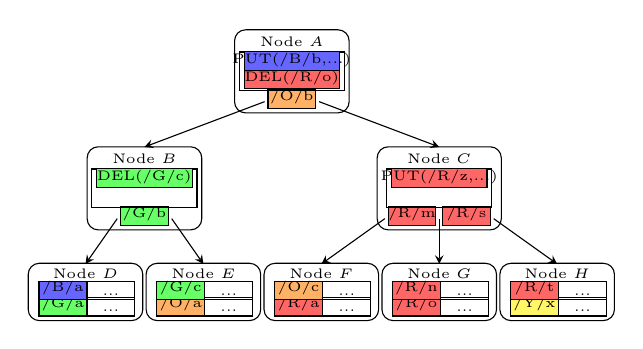
\begin{tikzpicture}[xscale=0.95, yscale=0.95]
        \node[anchor=south, rectangle, rounded corners, minimum height=.06\textwidth, minimum width=.12\textwidth, draw=black] at (0, 0) {};
        \node[anchor=south, font=\tiny] at (0, .036\textwidth) {Node $F$};
        \node[anchor=south, rectangle, minimum height=.015\textwidth, minimum width=.05\textwidth, draw=black, fill={red!60}] at (-.025\textwidth, .005\textwidth) {};
        \node[anchor=south, font=\tiny] at (-.025\textwidth, 0) {/R/a};
        \node[anchor=south, rectangle, minimum height=.015\textwidth, minimum width=.05\textwidth, draw=black] at (.028\textwidth, .005\textwidth) {};
        \node[anchor=south, font=\tiny] at (.028\textwidth, 0) {...};
        \node[anchor=south, rectangle, minimum height=.015\textwidth, minimum width=.05\textwidth, draw=black, fill={orange!60}] at (-.025\textwidth, .023\textwidth) {};
        \node[anchor=south, font=\tiny] at (-.025\textwidth, .018\textwidth) {/O/c};
        \node[anchor=south, rectangle, minimum height=.015\textwidth, minimum width=.05\textwidth, draw=black] at (.028\textwidth, .023\textwidth) {};
        \node[anchor=south, font=\tiny] at (.028\textwidth, .018\textwidth) {...};

        \node[anchor=south, rectangle, rounded corners, minimum height=.06\textwidth, minimum width=.12\textwidth, draw=black] at (.13\textwidth, 0) {};
        \node[anchor=south, font=\tiny] at (.13\textwidth, .036\textwidth) {Node $G$};
        \node[anchor=south, rectangle, minimum height=.015\textwidth, minimum width=.05\textwidth, draw=black, fill={red!60}] at (.105\textwidth, .005\textwidth) {};
        \node[anchor=south, font=\tiny] at (.105\textwidth, 0) {/R/o};
        \node[anchor=south, rectangle, minimum height=.015\textwidth, minimum width=.05\textwidth, draw=black] at (.158\textwidth, .005\textwidth) {};
        \node[anchor=south, font=\tiny] at (.158\textwidth, 0) {...};
        \node[anchor=south, rectangle, minimum height=.015\textwidth, minimum width=.05\textwidth, draw=black, fill={red!60}] at (.105\textwidth, .023\textwidth) {};
        \node[anchor=south, font=\tiny] at (.105\textwidth, .018\textwidth) {/R/n};
        \node[anchor=south, rectangle, minimum height=.015\textwidth, minimum width=.05\textwidth, draw=black] at (.158\textwidth, .023\textwidth) {};
        \node[anchor=south, font=\tiny] at (.158\textwidth, .018\textwidth) {...};

        \node[anchor=south, rectangle, rounded corners, minimum height=.06\textwidth, minimum width=.12\textwidth, draw=black] at (.26\textwidth, 0) {};
        \node[anchor=south, font=\tiny] at (.26\textwidth, .036\textwidth) {Node $H$};
        \node[anchor=south, rectangle, minimum height=.015\textwidth, minimum width=.05\textwidth, draw=black, fill={yellow!60}] at (.235\textwidth, .005\textwidth) {};
        \node[anchor=south, font=\tiny] at (.235\textwidth, 0) {/Y/x};
        \node[anchor=south, rectangle, minimum height=.015\textwidth, minimum width=.05\textwidth, draw=black] at (.288\textwidth, .005\textwidth) {};
        \node[anchor=south, font=\tiny] at (.288\textwidth, 0) {...};
        \node[anchor=south, rectangle, minimum height=.015\textwidth, minimum width=.05\textwidth, draw=black, fill={red!60}] at (.235\textwidth, .023\textwidth) {};
        \node[anchor=south, font=\tiny] at (.235\textwidth, .018\textwidth) {/R/t};
        \node[anchor=south, rectangle, minimum height=.015\textwidth, minimum width=.05\textwidth, draw=black] at (.288\textwidth, .023\textwidth) {};
        \node[anchor=south, font=\tiny] at (.288\textwidth, .018\textwidth) {...};

        \node[anchor=south, rectangle, rounded corners, minimum height=.06\textwidth, minimum width=.12\textwidth, draw=black] at (-.13\textwidth, 0) {};
        \node[anchor=south, font=\tiny] at (-.13\textwidth, .036\textwidth) {Node $E$};
        \node[anchor=south, rectangle, minimum height=.015\textwidth, minimum width=.05\textwidth, draw=black, fill={orange!60}] at (-.155\textwidth, .005\textwidth) {};
        \node[anchor=south, font=\tiny] at (-.155\textwidth, 0) {/O/a};
        \node[anchor=south, rectangle, minimum height=.015\textwidth, minimum width=.05\textwidth, draw=black] at (-.102\textwidth, .005\textwidth) {};
        \node[anchor=south, font=\tiny] at (-.102\textwidth, 0) {...};
        \node[anchor=south, rectangle, minimum height=.015\textwidth, minimum width=.05\textwidth, draw=black, fill={green!60}] at (-.155\textwidth, .023\textwidth) {};
        \node[anchor=south, font=\tiny] at (-.155\textwidth, .018\textwidth) {/G/c};
        \node[anchor=south, rectangle, minimum height=.015\textwidth, minimum width=.05\textwidth, draw=black] at (-.102\textwidth, .023\textwidth) {};
        \node[anchor=south, font=\tiny] at (-.102\textwidth, .018\textwidth) {...};

        \node[anchor=south, rectangle, rounded corners, minimum height=.06\textwidth, minimum width=.12\textwidth, draw=black] at (-.26\textwidth, 0) {};
        \node[anchor=south, font=\tiny] at (-.26\textwidth, .036\textwidth) {Node $D$};
        \node[anchor=south, rectangle, minimum height=.015\textwidth, minimum width=.05\textwidth, draw=black, fill={green!60}] at (-.285\textwidth, .005\textwidth) {};
        \node[anchor=south, font=\tiny] at (-.285\textwidth, 0) {/G/a};
        \node[anchor=south, rectangle, minimum height=.015\textwidth, minimum width=.05\textwidth, draw=black] at (-.232\textwidth, .005\textwidth) {};
        \node[anchor=south, font=\tiny] at (-.232\textwidth, 0) {...};
        \node[anchor=south, rectangle, minimum height=.015\textwidth, minimum width=.05\textwidth, draw=black, fill={blue!60}] at (-.285\textwidth, .023\textwidth) {};
        \node[anchor=south, font=\tiny] at (-.285\textwidth, .018\textwidth) {/B/a};
        \node[anchor=south, rectangle, minimum height=.015\textwidth, minimum width=.05\textwidth, draw=black] at (-.232\textwidth, .023\textwidth) {};
        \node[anchor=south, font=\tiny] at (-.232\textwidth, .018\textwidth) {...};

        \node[anchor=south, rectangle, rounded corners, minimum height=.087\textwidth, minimum width=.12\textwidth, draw=black] at (-.195\textwidth, .1\textwidth) {};
        \node[anchor=south, font=\tiny] at (-.195\textwidth, .163\textwidth) {Node $B$};
        \node[anchor=south, rectangle, minimum height=.015\textwidth, minimum width=.05\textwidth, draw=black, fill={green!60}] at (-.195\textwidth, .105\textwidth) {};
        \node[anchor=south, font=\tiny] at (-.195\textwidth, .1\textwidth) {/G/b};
        \node[anchor=south, rectangle, minimum height=.04\textwidth, minimum width=.11\textwidth, draw=black] at (-.195\textwidth, .125\textwidth) {};
        \node[anchor=south, rectangle, minimum height=.015\textwidth, minimum width=.1\textwidth, draw=black, fill={green!60}] at (-.195\textwidth, .147\textwidth) {};
        \node[anchor=south, font=\tiny] at  (-.195\textwidth, .141\textwidth) {DEL(/G/c)};

        \node[anchor=south, rectangle, rounded corners, minimum height=.087\textwidth, minimum width=.13\textwidth, draw=black] at (.13\textwidth, .1\textwidth) {};
        \node[anchor=south, font=\tiny] at (.13\textwidth, .163\textwidth) {Node $C$};
        \node[anchor=south, rectangle, minimum height=.015\textwidth, minimum width=.05\textwidth, draw=black, fill={red!60}] at (.1\textwidth, .105\textwidth) {};
        \node[anchor=south, font=\tiny] at (.1\textwidth, .1\textwidth) {/R/m};
        \node[anchor=south, rectangle, minimum height=.015\textwidth, minimum width=.05\textwidth, draw=black, fill={red!60}] at (.16\textwidth, .105\textwidth) {};
        \node[anchor=south, font=\tiny] at (.16\textwidth, .1\textwidth) {/R/s};
        \node[anchor=south, rectangle, minimum height=.04\textwidth, minimum width=.11\textwidth, draw=black] at (.13\textwidth, .125\textwidth) {};
        \node[anchor=south, rectangle, minimum height=.015\textwidth, minimum width=.1\textwidth, draw=black, fill={red!60}] at (.13\textwidth, .147\textwidth) {};
        \node[anchor=south, font=\tiny] at  (.13\textwidth, .141\textwidth) {PUT(/R/z,...)};

        \node[anchor=south, rectangle, rounded corners, minimum height=.087\textwidth, minimum width=.12\textwidth, draw=black] at (-.0325\textwidth, .229\textwidth) {};
        \node[anchor=south, font=\tiny] at (-.0325\textwidth, .292\textwidth) {Node $A$};
        \node[anchor=south, rectangle, minimum height=.015\textwidth, minimum width=.05\textwidth, draw=black, fill={orange!60}] at (-.0325\textwidth, .234\textwidth) {};
        \node[anchor=south, font=\tiny] at (-.0325\textwidth, .229\textwidth) {/O/b};
        \node[anchor=south, rectangle, minimum height=.04\textwidth, minimum width=.11\textwidth, draw=black] at (-.0325\textwidth, .254\textwidth) {};
        \node[anchor=south, rectangle, minimum height=.015\textwidth, minimum width=.1\textwidth, draw=black, fill={red!60}] at (-.0325\textwidth, .256\textwidth) {};
        \node[anchor=south, font=\tiny] at  (-.0325\textwidth, .25\textwidth) {DEL(/R/o)};
        \node[anchor=south, rectangle, minimum height=.015\textwidth, minimum width=.1\textwidth, draw=black, fill={blue!60}] at (-.0325\textwidth, .276\textwidth) {};
        \node[anchor=south, font=\tiny] at  (-.0325\textwidth, .27\textwidth) {PUT(/B/b,...)};

        \draw[->, >=stealth] (-.225\textwidth, .113\textwidth) -- (-.26\textwidth, .063\textwidth);
        \draw[->, >=stealth] (-.165\textwidth, .113\textwidth) -- (-.13\textwidth, .063\textwidth);
        \draw[->, >=stealth] (.13\textwidth, .113\textwidth) -- (.13\textwidth, .063\textwidth);
        \draw[->, >=stealth] (.19\textwidth, .113\textwidth) -- (.26\textwidth, .063\textwidth);
        \draw[->, >=stealth] (.07\textwidth, .113\textwidth) -- (0, .063\textwidth);
        \draw[->, >=stealth] (-.0625\textwidth, .242\textwidth) -- (-.195\textwidth, .192\textwidth);
        \draw[->, >=stealth] (-.0025\textwidth, .242\textwidth) -- (.13\textwidth, .192\textwidth);
    \end{tikzpicture}
    \caption[A \bet]{\label{fig:bet} A \bet.}
\end{figure}

\begin{table}[t]
    \centering
    \begin{tabular}{c | c c c}
        \hline
        Data Structure & Insert & Point Query & Range Query \\
        \hline
        \hline
        \btree & $O(log_{B}{N})$ & $O(log_{B}{N})$ & $O(log_{B}{N} + k/B)$\\
        \hline
        \bet & $O({log_{B}{N}}/{\varepsilon B^{1 - \varepsilon}})$ & $O({log_{B}{N}}/{\varepsilon})$ & $O({log_{B}{N}}/{\varepsilon} + k/B)$ \\
        \hline
        \bet ($\varepsilon=0.5$) & $O(log_{B}{N}/{\sqrt{B}})$ & $O(log_{B}{N})$ & $O(log_{B}{N} + k/B)$ \\
        \hline
    \end{tabular}
    \caption[The asymptotic IO costs of \btrees and \bets]{\label{tab:betbtree}
        The asymptotic IO costs of \btrees and \bets.}
\end{table}

\bets are asymptotically faster than \btrees, as summarized in
Table~\ref{tab:betbtree}.
Consider a \btree with $N$ key/value pairs and in which each node can hold
$B$ keys
(for simplicity, assume keys have constant size and that the value associated
with each key has negligible size).
The tree has fanout $B$, so its height is $O(log_{B}{N})$.
Inserts and point queries need to fetch all nodes along the root-to-leaf path,
resulting in $O(log_{B}{N})$ IOs.
A range query for $k$ key/value pairs requires $O(log_{B}{N} + k/B)$ IOs.

For comparison, a \bet with node size $B$ has fanout $B^{\varepsilon}$, where
$0 < \varepsilon \leq 1$.
Therefore, pivot keys in a non-leaf node consume $B^{\varepsilon}$ space and
the remaining $(B - B^{\varepsilon})$ space is used for buffers.
As a result, the \bet has height $O(log_{B}{N}/\varepsilon)$.
A point query fetches all nodes along the root-to-leaf path with
$O(log_{B}{N}/\varepsilon)$ IOs and a range query for $k$ key/value pairs
requires $O({log_{B}{N}}/{\varepsilon} + k/B)$ IOs.
On the other hand, the cost of an insert consists of injecting the message into
the root node with $O(1)$ IO and flushing the message down at each level.
In each flush, \bets has $O(B - B^{\varepsilon})$ messages and $B^{\varepsilon}$
children.
Thus, at leave one child can receive at least
$O((B - B^{\varepsilon})/B^{\varepsilon}) = O(B^{1 - \varepsilon})$ messages.
Therefore, the amortized cost of an insert in one flush is
$O(1/B^{1 - \varepsilon})$.
As the insert must be flushed $O(log_{B}{N}/\varepsilon)$ times, the amortized
cost of the insert is $O({log_{B}{N}}/{\varepsilon B^{1 - \varepsilon}})$.
A \bet with $\varepsilon = 1$ is equivalent to a \btree.
And if $\varepsilon = 1/2$, the point and range query costs of the \bet
become $O(log_{B}{N})$ and $O(log_{B}{N} + k/B)$, which is the same as a \btree,
but the insert cost becomes $O(log_{B}{N}/{\sqrt{B}})$, which is faster by a
factor of $\sqrt{B}$.

One important change in \bets from \btrees is the asymmetric IO costs for
point queries and inserts.
In \btrees, if an application wants to update the old value associated with a
key, it performs a point query to get the old value and then issues an insert
with the updated value.
Because both operations take $O(log_{B}{N})$ IOs, the total cost remains
$O(log_{B}{N})$.
However, in \bets, the query cost is $O(log_{B}{N}/\varepsilon)$ IOs while the
insert cost is $O({log_{B}{N}}/{\varepsilon B^{1 - \varepsilon}})$.
Performing a query before an insert degrades the total cost to
$O(log_{B}{N}/\varepsilon)$ IOs.

To avoid this read-before-write problem, \bets support ``upsert'' operations.
An upsert injects a message with the key and a delta into the buffer of the root
node.
When the upsert message is flushed to the leaf, it updates the old value
associated with the key with a user-specified function and the delta in the
message.
With upsert messages, queries need to compute value on the fly.
However, this doesn't change the IO costs of queries.
On the other hand, updating an old value becomes as fast as an insert.

\section{Full-path-indexed \betrfs}
\label{sec:fpi}

\begin{figure}[t]
    \centering
    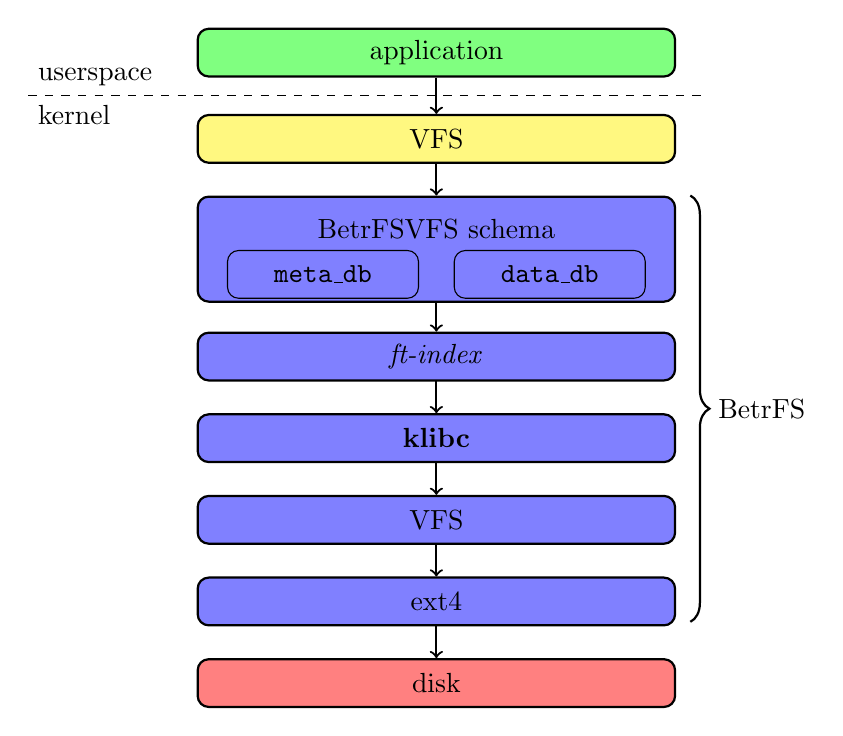
\begin{tikzpicture}[yscale=0.95, xscale=0.95]
    \draw[thick, ->] (0, .04\textwidth) -- (0, 0) node [anchor=north, rectangle, rounded corners, text centered, minimum height=.05\textwidth, minimum width=.5\textwidth, draw=black, fill=red!50] {disk};
    \draw[thick, ->] (0, .13\textwidth) -- (0, .09\textwidth) node [anchor=north, rectangle, rounded corners, text centered, minimum height=.05\textwidth, minimum width=.5\textwidth, draw=black, fill=blue!50] {ext4};
    \draw[thick, ->] (0, .22\textwidth) -- (0, .18\textwidth) node [anchor=north, rectangle, rounded corners, text centered, minimum height=.05\textwidth, minimum width=.5\textwidth, draw=black, fill=blue!50] {VFS};
    \draw[thick, ->] (0, .31\textwidth) -- (0, .27\textwidth) node [anchor=north, rectangle, rounded corners, text centered, minimum height=.05\textwidth, minimum width=.5\textwidth, draw=black, fill=blue!50] {\klibc};
    \draw[thick, ->] (0, .4\textwidth) -- (0, .36\textwidth) node [anchor=north, rectangle, rounded corners, text centered, minimum height=.05\textwidth, minimum width=.5\textwidth, draw=black, fill=blue!50] {\fti};
    \draw[thick, ->] (0, .55\textwidth) -- (0, .51\textwidth) node [anchor=north, rectangle, rounded corners, text centered, minimum height=.11\textwidth, minimum width=.5\textwidth, draw=black, fill=blue!50] {};
    \node [anchor=north, rectangle, rounded corners, text centered, minimum height=.05\textwidth, minimum width=.2\textwidth, draw=black, fill=blue!50] at (.125\textwidth, .45\textwidth) {\ddb};
    \node [anchor=north, rectangle, rounded corners, text centered, minimum height=.05\textwidth, minimum width=.2\textwidth, draw=black, fill=blue!50] at (-.125\textwidth, .45\textwidth) {\mdb};
    \node [anchor=north, text centered, minimum height=.05\textwidth] at (0, .50\textwidth) {\betrfs VFS schema};
    \draw[thick, ->] (0, .64\textwidth) -- (0, .60\textwidth) node [anchor=north, rectangle, rounded corners, text centered, minimum height=.05\textwidth, minimum width=.5\textwidth, draw=black, fill=yellow!50] {VFS};
    \node[anchor=south, rectangle, rounded corners, text centered, minimum height=.05\textwidth, minimum width=.5\textwidth, draw=black, thick, fill=green!50] at (0, .64\textwidth) {application};
    \draw[dashed] (-.45\textwidth, .62\textwidth) -- (.3\textwidth, .62\textwidth);
    \node[anchor=south west] at (-.45\textwidth, .62\textwidth) {userspace};
    \node[anchor=north west] at (-.45\textwidth, .62\textwidth) {kernel};
    \draw[decorate, decoration={brace,amplitude=.02\textwidth,mirror}, thick] (.28\textwidth, .04\textwidth) -- (.28\textwidth, .51\textwidth);
    \node[anchor=west,text centered] at (.3\textwidth, .275\textwidth) {\betrfs};
    \end{tikzpicture}
    \caption[The \betrfs architecture]{\label{fig:betrfs}
        The \betrfs architecture.}
\end{figure}

\betrfs~\citep{betrfs1,betrfs1tos} is a Linux in-kernel file
system built upon \fti~\citep{fti}, a key/value store that implements \bets and
exposes a key/value interface similar to BerkelyDB.
The architecture of \betrfs is shown in Figure~\ref{fig:betrfs}.
\betrfs interacts with \fti through point operations, such as \texttt{put},
\texttt{get} and \texttt{del}, as well as range queries with cursors
(\texttt{c\_get} with DB\_SET\_RANGE and DB\_NEXT).
\betrfs also uses the transaction interface of \fti to execute multiple
operations atomically.
A redo log and periodic checkpoints (every 60 seconds) in \fti ensure that
changes can be made persistent on disk.

\Fti cannot be integrated into a Linux kernel module easily because
it is a userspace library that assumes libc functions and system calls.
\betrfs has a shim layer called \klibc that implements all functions \fti
requires.
Through this way, \betrfs can incorporate \fti into the kernel module without
modifying code in \fti.

\betrfs uses two key/value indexes to store the metadata and data in the file
system.
One \mdb maps full-paths to \texttt{struct stat} structures.
Another \ddb maps (full-path and block number) to 4KB blocks.
When the VFS (Virtual File System) needs metadata, \betrfs queries
the \mdb with the full-path and constructs the corresponding inode
from the \texttt{struct stat}.
Likewise, when a dirty inode needs to be written, the \texttt{struct stat} is
assembled from the inode and written to the \mdb with the
full-path key.
Blocks of a file are fetched and written by the full-path and the indexes of
blocks.
Although other block granularity is possible, 4KB is the natural block size
because it is the same as the page size in the Linux page cache.

\betrfs can write to a block without fetching the old block to memory, avoiding
expensive read-before-write described in Section~\ref{sec:bet}.
Conventional file systems must read the old block from the disk to the page
cache before writing to that block (a complete overwrite can be done without
fetching the old block, but it is not implemented in any file system).
However, \bets have asymmetric read and write costs, so read-before-write should
be avoided.
In \betrfs, if the corresponding block is not in memory, an upsert message,
which describes the offset, length and content of this write, is injected into
the \bet.
When this message is flushed to the leaf, the change is applied to the old
block.

Full-path indexing ensures locality even with file system aging~\citep{betrfs3}.
After \betrfs fetches one block of a file from the disk, all nodes along the
root-to-leaf path are present in memory.
And with full-path indexing, all keys under one directory are contiguous in the
keyspace, which means a subsequent fetch of some other block in the same file or
another file under than same directory is likely to be resolved in memory,
which significantly increases performance and IO efficiency.

The first implementation of \betrfs (\betrfsOne) shows great random write
performance.
Recursive greps run 3.77x faster than in the best standard file system.
File creation runs 12.54x faster.
Small, random writes to a file run 68.24x faster~\citep{betrfs1tos}.

However, namespace operations have predictably miserable performance in
\betrfsOne.
Deleting and renaming a Linux source directory takes 46.14 and 21.17 seconds,
respectively, because the file system has to call one or more key/value store
operations for each key.
The deleting problem is fixed by a range-delete message that nullifies all
messages within a range, but the renaming problem remains difficult.

\section{Relative-path-indexed \betrfs}
\label{sec:rpi}

\begin{figure}[t]
    \begin{subfigure}{.5\textwidth}
        \centering
        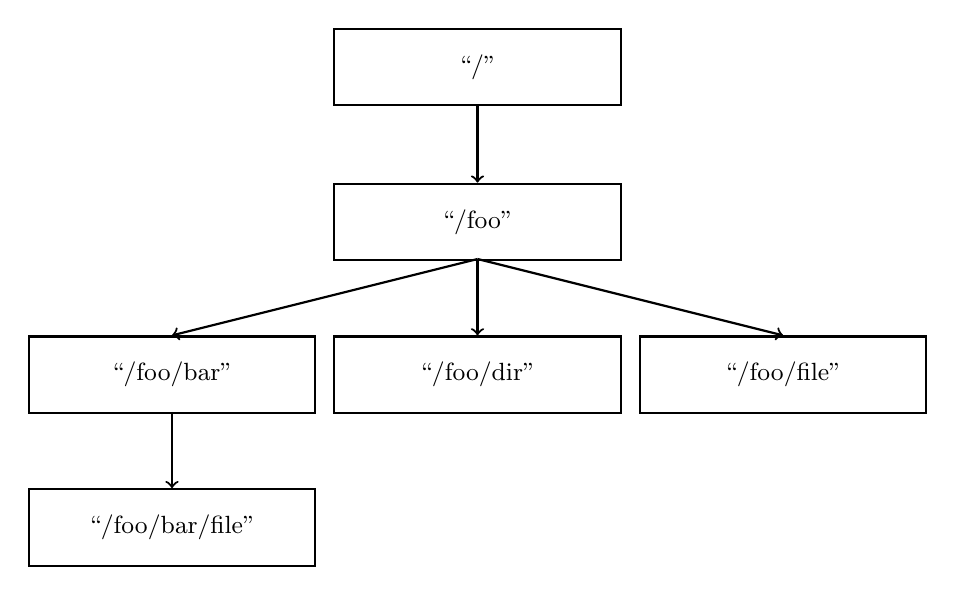
\begin{tikzpicture}{xscale=0.95,yscale=0.95}
            \draw[thick, ->] (0, .08\textwidth) -- (0, 0) node [anchor=north, rectangle, text centered, minimum height=.08\textwidth, minimum width=.3\textwidth, draw=black, font=\small] {``/foo/bar/file''};
            \draw[thick, ->] (.32\textwidth, .24\textwidth) -- (0, .16\textwidth) node [anchor=north, rectangle, text centered, minimum height=.08\textwidth, minimum width=.3\textwidth, draw=black, font=\small] {``/foo/bar''};
            \draw[thick, ->] (.32\textwidth, .24\textwidth) -- (.32\textwidth, .16\textwidth) node [anchor=north, rectangle, text centered, minimum height=.08\textwidth, minimum width=.3\textwidth, draw=black, font=\small] {``/foo/dir''};
            \draw[thick, ->] (.32\textwidth, .24\textwidth) -- (.64\textwidth, .16\textwidth) node [anchor=north, rectangle, text centered, minimum height=.08\textwidth, minimum width=.3\textwidth, draw=black, font=\small] {``/foo/file''};
            \draw[thick, ->] (.32\textwidth, .4\textwidth) -- (.32\textwidth, .32\textwidth) node [anchor=north, rectangle, text centered, minimum height=.08\textwidth, minimum width=.3\textwidth, draw=black, font=\small] {``/foo''};
            \node [anchor=south, rectangle, text centered, minimum height=.08\textwidth, minimum width=.3\textwidth, draw=black, thick, font=\small] at (.32\textwidth, .4\textwidth) {``/''};
        \end{tikzpicture}
        \caption{\label{subfig:FPI} Full-path indexing.}
    \end{subfigure}
    \begin{subfigure}{.5\textwidth}
        \centering
        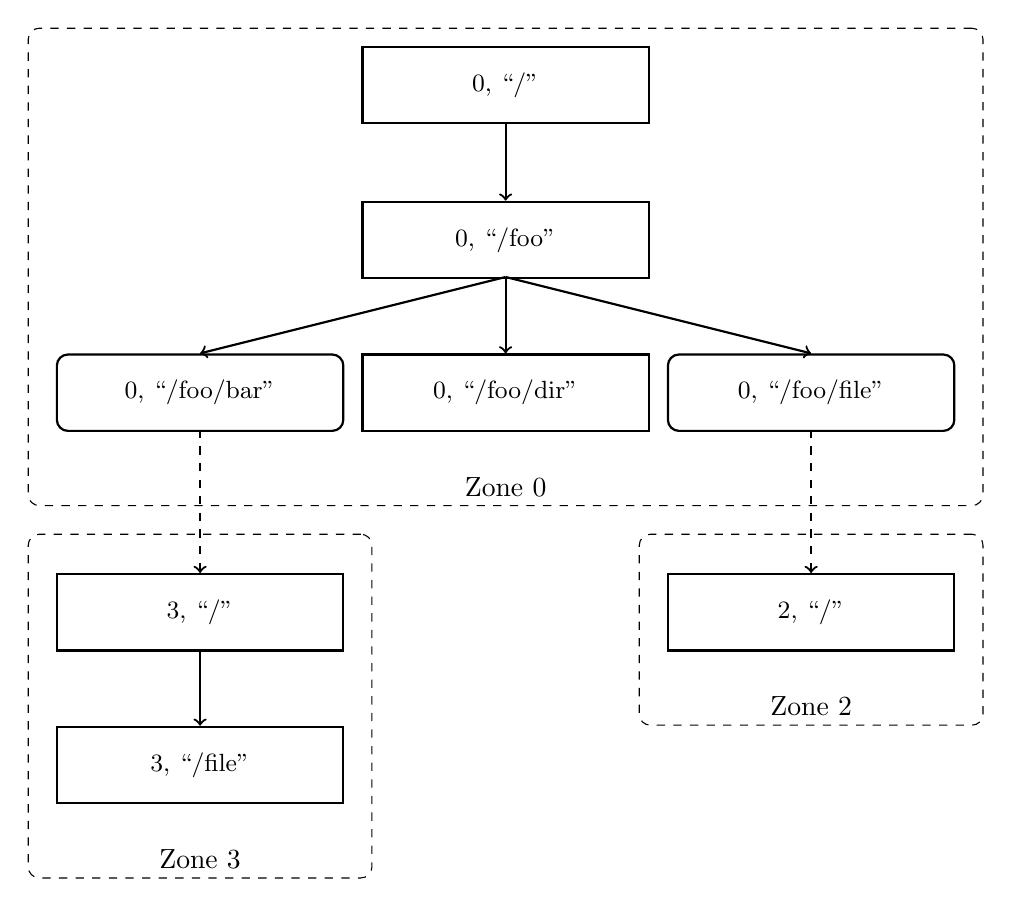
\begin{tikzpicture}{xscale=0.95,yscale=0.95}
            \node [anchor=south, rectangle, rounded corners, minimum height=.50\textwidth, minimum width=\textwidth, draw=black, dashed] at (.32\textwidth, 0) {};
            \node [anchor=south] at (.32\textwidth, 0) {Zone 0};
            \draw[thick, ->] (.32\textwidth, .24\textwidth) -- (0, .16\textwidth) node [anchor=north, rectangle, rounded corners, text centered, minimum height=.08\textwidth, minimum width=.3\textwidth, draw=black, font=\small] {0, ``/foo/bar''};
            \draw[thick, ->] (.32\textwidth, .24\textwidth) -- (.32\textwidth, .16\textwidth) node [anchor=north, rectangle, text centered, minimum height=.08\textwidth, minimum width=.3\textwidth, draw=black, font=\small] {0, ``/foo/dir''};
            \draw[thick, ->] (.32\textwidth, .24\textwidth) -- (.64\textwidth, .16\textwidth) node [anchor=north, rectangle, rounded corners, text centered, minimum height=.08\textwidth, minimum width=.3\textwidth, draw=black, font=\small] {0, ``/foo/file''};
            \draw[thick, ->] (.32\textwidth, .4\textwidth) -- (.32\textwidth, .32\textwidth) node [anchor=north, rectangle, text centered, minimum height=.08\textwidth, minimum width=.3\textwidth, draw=black, font=\small] {0, ``/foo''};
            \node [anchor=south, rectangle, text centered, minimum height=.08\textwidth, minimum width=.3\textwidth, draw=black, thick, font=\small] at (.32\textwidth, .4\textwidth) {0, ``/''};
            \node [anchor=south, rectangle, rounded corners, minimum height=.36\textwidth, minimum width=.36\textwidth, draw=black, dashed] at (0, -.39\textwidth) {};
            \node [anchor=south] at (0, -.39\textwidth) {Zone 3};
            \node [anchor=north, rectangle, text centered, minimum height=.08\textwidth, minimum width=.3\textwidth, draw=black, thick, font=\small] at (0, -.07\textwidth) {3, ``/''};
            \draw[thick, ->] (0, -.15\textwidth) -- (0, -.23\textwidth) node [anchor=north, rectangle, text centered, minimum height=.08\textwidth, minimum width=.3\textwidth, draw=black, font=\small] {3, ``/file''};
            \node [anchor=south, rectangle, rounded corners, minimum height=.2\textwidth, minimum width=.36\textwidth, draw=black, dashed] at (.64\textwidth, -.23\textwidth) {};
            \node [anchor=south] at (.64\textwidth, -.23\textwidth) {Zone 2};
            \node [anchor=north, rectangle, text centered, minimum height=.08\textwidth, minimum width=.3\textwidth, draw=black, thick, font=\small] at (.64\textwidth, -.07\textwidth) {2, ``/''};
            \draw[thick, dashed, ->] (0, .08\textwidth) -- (0, -.07\textwidth);
            \draw[thick, dashed, ->] (.64\textwidth, .08\textwidth) -- (.64\textwidth, -.07\textwidth);
        \end{tikzpicture}
        \caption{\label{subfig:RPI} Relative-path indexing.}
    \end{subfigure}
    \caption[Full-path indexing and relative-path indexing]{\label{fig:FPIRPI}
        Full-path indexing and relative-path indexing.}
\end{figure}

Relative-path-indexed \betrfs~\citep{betrfs2,betrfs2tos} backed away from
full-path indexing and introduced relative-path indexing,
which is also called zoning.
Relative-path indexing partitions the directory hierarchy into zones.
Each zone has a zone ID (the root zone has zone ID 0), which is analogous to an
inode number, and a single root file or directory.
All file or directory in a zone is indexed relative to the zone root.
If the file or directory is the root of another zone, the entry contains that
zone ID to redirect queries.

Figure~\ref{fig:FPIRPI} shows an example of the same directory hierarchy under
full-path indexing and relative-path indexing.
In Figure~\ref{subfig:RPI}, when querying the key/value store for file
``/foo/file'' with key (0, ``/foo/file''), the file system gets a special value
indicating it is the root of Zone 2.
Subsequently, the file system queries the key/value store with key (2, ``/'')
and gets the right value.
Similary, the file system notices the key for directory ``/foo/bar'' is
(3, ``/'').
Therefore, when querying for file ``/foo/bar/file'', it uses key (3, ``/file'').

\newcommand{\addTokubenchZonePlot}[1]
{
    \addplot[
        color=\pgfkeysvalueof{/fs-colors/#1},
        line width=0.75pt,
        mark=\pgfkeysvalueof{/fs-marks/#1},
    ]
    plot[
    ]
    table[
    ]
    {./data/tokuzone/#1.csv};
    \addlegendentry{\pgfkeysvalueof{/fs-names/#1}}
}

\begin{figure}[t]
    \centering
    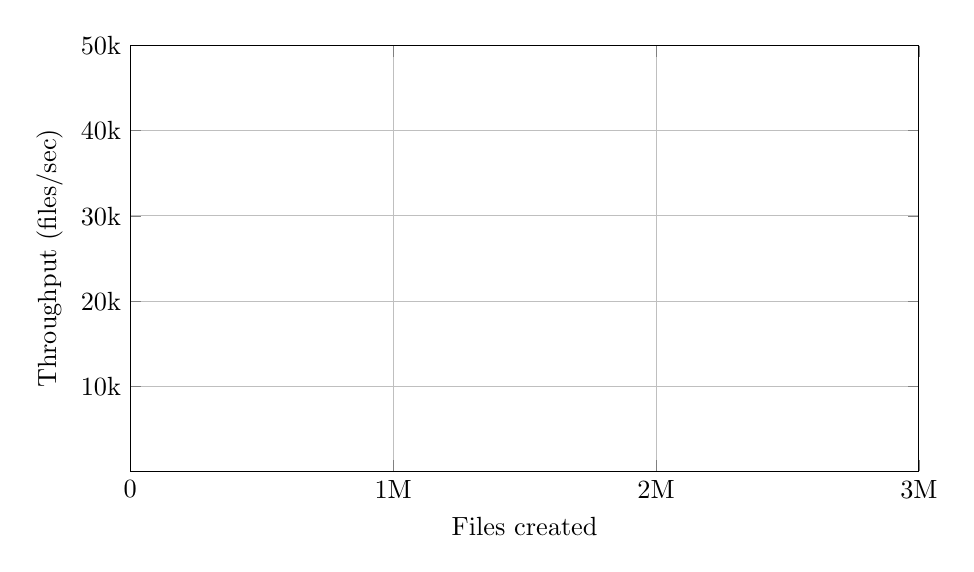
\begin{tikzpicture}[yscale=0.95,xscale=0.95]
        \begin{axis}[
            xlabel={Files created},
            ylabel={Throughput (files/sec)},
            xmin=0,
            xmax=3000000,
            ymin=10,
            ymax=50000,
            mark repeat=10,
            xtick={0,1000000,2000000,3000000},
            xticklabels={0,1M,2M,3M},
            ytick={10000,20000,30000,40000,50000},
            yticklabels={10k,20k,30k,40k,50k},
            grid=major,
            scaled x ticks=false,
            scaled y ticks=false,
            legend cell align=left,
            transpose legend,
            height=.6\linewidth,
            width=\linewidth,
        ]
        \addTokubenchZonePlot{betrfs3};
        \addTokubenchZonePlot{betrfs3-max};
        \end{axis}
    \end{tikzpicture}
    \caption[Zone maintainance cost in TokuBench benchmark]{Cumulative file creation
        throughput during the Tokubench benchmark (higher is better).
        Compared to \betrfsThree with one zone, \betrfsThree has a sudden
        performance drop because of zone splitting.}
    \label{fig:tokuzone}
\end{figure}

Relative-path indexing tries to balance locality and rename performance through
a target zone size.
Larger zone size means better locality because full-path indexing is still
maintained within the zone.
Smaller zone size imposes a lower bound on rename latency
because no rename needs to mutate more key/value pairs than in a zone.

\betrfsTwo adopts relative-path-indexing with a default zone size 128KiB.
Relative-path indexing made renames on \betrfsTwo almost as fast as inode-based
file system and recursive-directory traversals almost as fast as \betrfsOne.

However, relative-path indexing also imposes zone maintenance costs on other
file system operations.
For instance, in Figure~\ref{fig:tokuzone},
two-thirds of the way through the TokuBench benchmark,
\betrfsThree (\betrfsThree is \betrfsTwo with some bug fixes) shows a sudden,
precipitous drop in cumulative throughput for small file creation,
because the file system performs a huge amount of zone splitting.
On the contrary, \betrfsThree with an infinite zone size (marked as \betrfsThree
with one zone) has a smooth curve throughout the benchmark.

Furthermore, relative-path indexing also has bad worst-case performance.
It is possible to construct arrangements of nested directories that will each
reside in their own zone.
Reading a file in the deepest directory will require reading one zone per
directory (each withits own I/O).
Such a pathological worst case is not possible with full-path indexing in a
\bet, and an important design goal for \betrfs is keeping a reasonable bound on
the worst cases.

\section{Summary}

\betrfs is a general file system designed for all operations, with a particular
focus on random writes and locality.
The underlying data structure, \bets, performs random writes faster than \btrees
by cascading writes in batches.
The full-path indexing schema of \betrfsOne ensures good locality, while making
renames slow.
The relative-path indexing schema of \betrfsTwo enables fast renames,
but imposes additional costs on other operations.



\chapter{Renaming}
\label{chap:rename}

Renaming

\section{Tree surgery}

This section describes our approach to renaming a directory or large file via
changes within the \bet, such that most of the data physically moved (or even
accessed) on disk.
Files that are smaller than 4 MiB reside in at most two leaves.
We therefore move them by copying.
We reserve tree surgery only for larger files and, for simplicity of the
prototype, directories of any size.

For the sake of discussion, we assume that a rename is moving a source file over
an existing destination file;
the process would work similarly (but avoid some work) in the case where the
destination file does not exist.
Our implementation respects Portable Operating System Interface (POSIX)
restrictions for directories
(i.e., you cannot rename over a non-empty destination directory),
but our technique could easily support different directory rename semantics.
In the case of renaming over a file, where a rename implicitly deletes the
destination file, we use transactions in the \bet to insert both a range delete
of the destination and a range rename of the source;
these messages are applied atomically.

This section also operates primarily at the \bet level, not the directory
namespace.  Unless otherwise noted, pointers are pointers within the \bet.

A \bet node covers a key $k$ if and only if the node is on $k$'s search
path. Note that a node covers $k$, even if $k$ is not a key in the
tree.  Each \bet node thus covers a range of keys defined by a max
and min key.  For most nodes, the max and min are the
pivots bracketing the pointer from the parent to the child.  But for
some nodes, such as the first or last child of a parent, the range
will be defined by a pivot at the parent and a pivot at a more distant ancestor.

In renaming a file, the goal is to capture a range of contiguous keys and
logically move these key/value pairs to a different point in the tree.
For anything large enough to warrant using this rename approach,
some \bet nodes will exclusively store messages or key/value pairs
for the source or destination.
Some nodes may also include unrelated messages or key/value pairs
before and after this key range in sort order;
within the \bet these nodes will be along the left and right side of the nodes
that store only the messages or key/value pairs of interest.

An important abstraction for tree surgery is the \textbf{LCA}
(Lowest Common Ancestor) of two keys: the LCA is the \bet node lowest in the
tree on the search path for both keys (and hence including all keys in between).
During a range rename, the source and destination key ranges will each have an
LCA, and their LCAs may be the same node.

The first step in tree surgery is to find the source LCA and destination LCA.
In the process of identifying the LCAs, we also flush any pending messages for
the source or destination key range, so that they are buffered at or below the
corresponding LCAs.

\paragraph{Slicing}  The second step is to slice out the source and destination
key ranges from any shared nodes.
The goal of slicing is to separate unrelated key-value pairs that are not being
moved but are packed into the same \bet node as the key ranges to be move.
Slicing uses the same  code used for standard \bet node splits, but slicing
divides the node at the slicing key rather than picking a key in the middle of
the node.
As a result, slicing may result in nodes that temporarily violate constraints on
target node size and fanout.
However, these are performance, not correctness, constraints, so we can let
queries continue concurrently, and we restore these invariants before completing
the rename.

\textbf{Figures Here.}

Our implementation requires that the source and destination LCA be at the same
height for the next step.
Thus, if the LCAs are not at the same level of the tree, we slice up to an
ancestor of the higher LCA.
The goal of this choice is to maintain the invariant that all \bet leaves be
at the same depth.

After this swap completes, and the locks are released,
new searches or updates for the destination will descend into the new subtree.

\paragraph{Healing}  Our \bet implementation maintains the
invariant that all internal nodes have between 4 and 16 children,
which bounds the height of the tree.  After the transplant completes,
however, there may be a number of in-memory \bet nodes at the fringe
around the source and destination that have fewer than 4 children.

We handle this situation by triggering a rebalancing within the tree.
Specifically, if a node has only one child, the slicing process will merge
it after completing the work of the rename.
After the transplant completes, there may be a number
of \bet nodes in memory at the fringe around the
source and destination that have fewer children than desired.
The healing process merges these smaller nodes back together,
using the same approach as a typical \bet merge.  At this point, it is also
possible that this could trigger a rebalancing within the tree.

One very important optimization we found as part of healing was to
agressively merge {\em stalks}, or new descendants of an LCA with
only a single child.
When the source and destination LCA are at different height, slicing
will creates some nodes with a single child.
Traversing these stalks undermines the logarithmic search time one would
expect from a tree, and created significant performance overheads.
After healing, we immediately merge nodes at the fringe
to a normal fanout in \bet.

\paragraph{Crash Consistency} \betrfs relies on three on-disk data structures to
ensure crash consistency: the trees, a block table indicating the disk blocks
used by the trees, and a write-ahead redo log. In general, \betrfs ensures crash
consistency by appending pending messages to the redo log and then applying
messages to the tree in a copy-on-write manner.
At periodic intervals (by default every 60 seconds), \betrfs ensures that there
is a consistent, sharp checkpoint of the tree on disk.
After a crash, \betrfs reads the last checkpointed tree and replays the redo log
after the checkpoint.
Range rename works within this framework.

A range rename is {\em logically applied} to the tree as soon as
(1) the range-rename message is added to the redo log and
(2) tree surgery locks the root of the tree.
The range rename is durable as soon as the redo log entry is written to disk.
If the system crashes after a range rename is logged, the recovery will see a
prefix of the message history that includes the range-rename message, and the
tree surgery will be redone in response to the range-rename message.
After both the tree surgery and the subsequent checkpoint of the tree complete,
there is no need to repeat the tree surgery after a crash.

We note that the current implementation does tree surgery immediately after the
message is placed in the redo log.
It is possible to batch range rename messages and apply them lazily,
but we leave this for future work.
As a result of this choice, however, there are fewer cases to reason about
in understanding crash consistency.

Tree surgery walks down the tree and locks the nodes along the path
hand-over-hand until either the source LCA or the destination LCA is reached.
Then, until tree surgery completes, all fringe nodes, the LCAs, and the parents
of LCAs are locked in memory and dirtied.
Upon tree surgery completion, these nodes will be unlocked.
Because the checkpoint process must grab the locks of all involved node before
writing them to disk,
no intermediate state of slicing will be exposed to a checkpoint.
Dirty nodes may be written back to disk, copy-on-write, before checkpointing
under memory pressure.
However, because the recovery process always starts from the last checkpoint and
the last block table in which these newly allocated nodes is not reachable,
these nodes with uncheckpointed state will be marked as free during crash
recovery.

If the system crashes after tree surgery begins but before surgery completes,
the recovery code will see a consistent checkpoint of the tree as it was
before the tree surgery.
The same is true if the system crashes after tree surgery but before dirty nodes
are written back to disk.
Because a checkpoint flushes all dirty nodes, if the system crashes after a
checkpoint, all nodes affected by tree surgery will be on disk.
We checked this functionality with crash recovery unit tests.
We ran the system in QEMU and crashed the system both before a rename completed
and before the rename log had been flushed;
we ensured that \betrfs restored the tree to the state before the tree surgery.

Tree surgery maintains the transactional properties of \betrfs.
It is performed at the commit stage of a range-rename transaction,
and thus aborting a range-rename transaction leaves no trace on the tree.
In the case of a crash, the tree surgery, which is encoded as a range-rename
message in the redo log, will be redone when the recovery process replays the
redo log.
The key to maintaining failure-atomicity of surgery is that all the involved
nodes must be locked in memory in the same batch to ensure the checkpoint has
a consistent snapshot of the tree at a point in time before or after,
but not during, the tree surgery.

At the file system level, \betrfs has similar crash consistency semantics to
metadata-only journaling in ext4.
The \bet implementation itself implements full data journaling, but \betrfs
allows file writes to be buffered in the VFS, weakening this guarantee
end-to-end.
Specifically, file writes may be buffered in the VFS caches, and are only logged
in the recovery journal once the VFS writes back a dirty page (e.g., upon an
{\tt fsync} or after a configurable period).
Changes to the directory tree structure, such as a {\tt rename} or {\tt mkdir}
are persisted to the log immediately.
Thus, in the common pattern of writing to a temporary file and then renaming it,
it is possible for the rename to appear in the log before the writes.
In this situation and in the absence of a crash, the writes will eventually be
logged with the correct, renamed key, as the in-memory inode will be up-to-date
with the correct \bet key.
If the system crashes, these writes can be lost; as with a metadata-journaled
file system, the developer must issue an {\tt fsync} before the {\tt rename} to
ensure the data is on disk.

\paragraph{Latency} A rename returns to the user once a log entry is in the
journal and the root node of the \bet is locked.
At this point, the rename has been applied in the VFS to in-memory metadata,
and as soon as the log is fsynced, the rename is durable.

We then hand off the rest of the rename work to two background threads
to do the cutting and healing.
The prototype in this paper only allows a backlog of one pending, large rename,
since we believe that concurrent renames are relatively infrequent.
The challenge in adding a rename work queue is ensuring consistency between the
work queue and the state of the tree.

\paragraph{Atomicity and Transactions}
The \bet in \betrfs implements multi-version concurrency control by augmenting
messages with a logical timestamp.
Messages updating a given key range are always applied in logical order.
Multiple messages can share a timestamp, giving them transactional semantics.

To ensure atomicity for a range rename, we create an MVCC ``hazard'':
read transactions ``before'' the rename must complete before the surgery
can proceed.
Tree nodes in \betrfs  are locked with reader-writer locks.
We write-lock tree nodes hand-over-hand, and left-to-right to identify
the LCAs.  Once the LCAs are locked, this serializes any new read or write
transactions until the rename completes.  The lock at the LCA creates
a ``barrier''---operations can complete ``above'' or ``below'' this lock
in the tree, although the slicing will wait for concurrent
transactions to complete before write-locking that node. Once the transplant
completes, the write-locks on the parents above LCAs are released.

In practice, \betrfs has a reader-writer lock in each in-memory inode to prevent
concurrent transactions from happening during a rename,
but this would be a concern in applying this technique to a general-purpose
key-value store or database that uses MVCC.

For simplicity, before the range rename is applied, we ensure that all messages
representing changes in the affected key range(s) that logically occurred before
the range rename are flushed below the LCA.
All messages that logically occur after the rename follow the new path through
the tree to the destination or source.
This strategy ensures that, when each message is flushed and applied, it sees a
point-in-time consistent view of the subtree.

\paragraph{Complexity} In the worst case, at most 4 slices are performed.
Slices go from the parent of the LCA to the leaf,
and nodes along this path are dirtied.
If the root of the tree is the LCA, a new root is inserted above the current
root for slicing.
These nodes will need to be read, if not in cache,
and written back to disk as part of the checkpointing process.
Therefore the number of IOs is at most proportional to the height of the \bet,
which is logarithmic in the size of the tree.

Let $N$ be the number of entries in a \bet, i.e., the number of files plus
directories in the metadata tree and the number of data blocks in the data tree.
Let $B$ be the size of a node.
And let $\varepsilon\in(0,1]$ be a design-time tuning parameter that adjusts the
fanout.
In the worst case, $O(\frac{\log_B{N}}{\varepsilon})$ (tree height)
I/Os will be performed  during a rename as a result of this design.

\section{Batched Key Updates}

After tree surgery completes, there will be a subtree where the keys
are not coherent with the new location in the tree.  As part of a
rename, the prefixes of all keys in this subtree need to be updated.
For example, suppose we execute \texttt{`mv /foo /bar'}.  After surgery,
any messages and
key/value pairs for file \texttt{/foo/file} will still have a key that
starts with \texttt{/foo}.  These keys need to be changed to begin
with \texttt{/bar}.  The particularly concerning case is when {\tt
  /foo} is a very large subtree and has interior nodes that would
otherwise be untouched by the tree surgery step; our goal is to leave
these nodes untouched as part of rename, and thus reduce the cost of
key changes from the size of the rename tree to the height of the
rename tree.

We note that full-path keys in our tree are highly redundant.
Our solution
reduces the work of changing keys by reducing the redundancy of how
keys are encoded in the tree.
Consider the prefix encoding for a sequence
of strings.  In this compression method, if two strings share a
substantial longest common prefix (lcp), then that lcp is only stored
once.  We apply this idea to \bets. % by changing the way that nodes store keys.
The lcp of all keys in a subtree is removed from the keys and stored in the
subtree's parent node.
We call this approach \textbf{key lifting} or
simply \textbf{lifting} for short.

At a high level, each parent in a lifted \bet stores
each child's common, lifted key prefix alongside the pointer to the child.
Child nodes only store differing key suffixes.
This approach encodes the complete key in the path taken to reach a given node.

This solution leaves nodes interior to the subtree to be unmodified as part of a range rename.
Specifically, part of finding an LCA during tree surgery ensures that the prefix to be renamed
is lifted into the parent.

One can then modify the prefix for a lifted subtree by only modifying the
parent node.
This solution
eliminates the need to change key and pivot prefixes in all nodes of a subtree.

Lifting requires a schema-level invariant that keys with a common prefix are adjacent
in the sort order.  As a simple example, if one uses {\tt memcmp} to compare keys (as \betrfs does),
then lifting will be correct.  This invariant ensures that, if there is a common prefix between any two pivot keys,
all keys in that child will have the same prefix, which can be safely lifted.
More formally:
\begin{invariant}
Let $T'$ be a subtree in a \bet with full-path indexing.  Let $p$ and
$q$ be the pivots that enclose $T'$.  That is, if $T'$ is not the first
or last child of its parent, then $p$ and $q$ are the enclosing pivots
in the parent of $T'$.  If $T'$ is the first child of its parent, then
$q$ is the first pivot and $p$ is the left enclosing pivot of the parent of $T'$.

Let $s$ be the longest common prefix of $p$ and $q$.  Then all keys
in $T'$ begin with $s$.
\end{invariant}

\textbf{Figures Here}

Reads can reconstruct the full key by concatenating prefixes during a
root-to-leaf traversal.  In principle, one need not store the lifted prefix ($s$)
in the tree, as it can be computed from the pivot keys.
In our implementation, we do memorize the lifted prefix for efficiency.

As messages are flushed to a child, they
are modified to remove the common prefix.
Similarly, node splits and merges ensure that
any common prefix between the pivot keys is lifted out.
It is possible for all of the keys in $T'$ to
share a common prefix that is longer than $s$,  but we only lift
$s$ because maintaining this amount of lifting hits a sweet spot: \textit{it
is enough to guarantee fast key updates during renames, but it
requires only local information at a parent and child  
during splits, merges, and insertions.}

Lifting  is completely transparent to the file system.
From the file system's perspective, it is still indexing data with a
key/value store that is keyed by full-path; the only difference from the file
system's perspective is that the key/value store completes some
operations faster.

\paragraph{Lifting and Renames}
In the case of renames, lifting dramatically reduces the work to update
keys.  During a rename from $a$ to $b$, we slice out a sub-tree
containing exactly those keys that have $a$ as a prefix.  By the
lifting invariant, the prefix $a$ will be lifted out of the sub-tree,
and the parent of the sub-tree will bound it between two pivots whose
common prefix is $a$ (or at least includes $a$---the pivots may have
an even longer common prefix).  After we perform the pointer swing,
the sub-tree will be bounded in its new parent by pivots that have $b$
as a common prefix.  Thus, by the lifting invariant, all future queries
will interpret all the keys in the sub-tree has having $b$ as a prefix.
Thus, with lifting, the pointer swing implicitly performs the batch key-prefix
replacement, completing the rename.

\paragraph{Complexity} During tree surgery, there is lifting work
along all nodes that are sliced or merged.  However, the number of
such nodes is at most proportional to the height of the tree.
Thus, the number of nodes that must be lifted after a rename is no more than
the nodes that must be sliced during tree surgery, and proportional to the height
of the tree.

After slicing out the subtree containing all the source keys involved in the rename,
the two source slicing keys become the two pivots bounding the source subtree in the
parent.
Because the common prefix of the two source slicing keys is the old prefix,
the old prefix is lifted from the source subtree.
Then, by inserting the subtree
to the new location that is bounded by two destination slicing keys with the new prefix,
all the keys in the subtree are updated immediately.
An end-to-end example of renaming is illustrated in Figure~\ref{fig:e2e}.
In this example, each slicing step lifts the old-prefix /red. By the time the slice reaches the LCA,
the old-prefix /red is lifted out of the entire subtree.

\section{Put them together}

\textbf{Figures Here}

\section{Summary}



\chapter{Cloning}
\label{chap:clone}

cloning


\chapter{Evaluation}
\label{chap:eval}

This chapter evaluates the performance of \betrfs with
range-rename (\betrfsFour) and \betrfs with range-clone (\betrfsFive).
The evaluation includes the following four aspects:
(1) performance of single file-system operations;
(2) performance of widely used applications;
(3) performance of renames;
(4) performance of clones.

\paragraph{Experimental Setup.}

All experimental results were collected on
a Dell Optiplex 790 with a 4-core 3.40 GHz Intel Core i7-2600 CPU,
4GB RAM,
and a 500 GB, 7200 SATA disk with a 4096-byte block size(Seagate Barracuda ST500DM002).
The system runs 64-bit Ubuntu server 14.04.05 on a USB stick to prevent
interference form the root file system.
\betrfsFour runs on a modified Linux-3.11.10 kernel that enlarges the size of the kernel stack,
while \betrfsFive and all other file systems run on Linux-4.9.142 kernel.
The evaluation uses ZFS 0.6.5.11 from \url{zfsonlinx.org} and
ext4, Btrfs, XFS and NILFS2 as parts of the Linux kernel.
Each experiment runs a minimum of 5 times and reports the median number.
Error bars indicate minimum and maximum numbers over all runs.
Similarly, error $\pm$ terms bound minimum and maximum numbers over all runs.
Unless noted, all benchmarks are cold-cache tests.

\section{Microbenchmarks}

\paragraph{Sequential writes and reads.}

We measure the throughput of sequentially writing and reading a file.
This benchmark first writes a 10-GiB file, 64 blocks at a time, with a
\texttt{fsync} to flush the file to disk.
Then, after cleaning the kernel page cache, the kernel reads the file from disk.

\newcommand{\addSeqPlot}[1]{
    \addplot[
        discard if not={fs}{#1},
        fill=\pgfkeysvalueof{/fs-colors/#1},
        nodes near coords=\pgfkeysvalueof{/fs-names/#1},
    ]
    plot[
        error bars/.cd,
        y dir=both, y explicit,
    ]
    table[
        x=op,
        y=median,
        y error plus expr=\thisrow{max}-\thisrow{median},
        y error minus expr=\thisrow{median}-\thisrow{min},
    ]
    {./data/seq_io.csv};
}

\begin{figure}[t]
    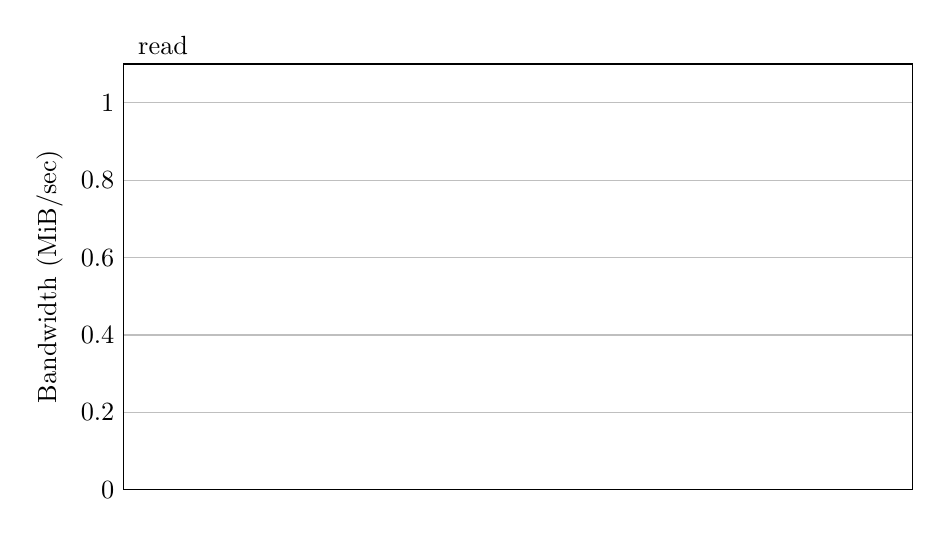
\begin{tikzpicture}[yscale=0.95, xscale=0.95]
        \begin{axis}[
                ybar,
                ymin=0,
                ylabel={Bandwidth (MiB/sec)},
                ymajorgrids=true,
                symbolic x coords={seq.write,seq.read},
                xtick={seq.write,seq.read},
                xticklabels={write,read},
                enlarge x limits=0.5,
                visualization depends on=y \as \rawy,
                xtick pos=right,
                major tick length=0in,
                xticklabel pos=right,
                nodes near coords style={font=\small,anchor=east,rotate=90,xshift=-\pgfplotsunitylength*\rawy,},
                height=.6\linewidth,
                width=\linewidth,
            ]
            \addSeqPlot{ext4};
            \addSeqPlot{btrfs};
            \addSeqPlot{xfs};
            \addSeqPlot{zfs};
            \addSeqPlot{nilfs2};
            \addSeqPlot{betrfs4};
            \addSeqPlot{betrfs5};
        \end{axis}
    \end{tikzpicture}
    \caption[Sequential-write and sequential-read benchmark]{\label{fig:seq_io}
        Bandwidth to sequentially read and write a 10 GiB file (higher is better).}
\end{figure}

Figure~\ref{fig:seq_io} shows the results.
Ext4, Btrfs, XFS performs sequential
writes close to disk bandwidth, while \betrfsFive, similar to NILFS2, is about
6.5\% slower than the fastest file system.
The performance increase of \betrfsFive from \betrfsFour is from preferential
splitting, which creates a pivot matching the maximum file data key the
beginning of the workload, avoiding further node relifting in subsequent node
splits.
For sequential reads, Ext4, Btrfs, XFS run at disk bandwidth, while \betrfsFive
is 19.1\% slower than the fastest file system, which is close to \betrfsFour
and NILFS2.
\betrfs reads a leaf, which is about 4 MiB in size, each time, while
extent-based file systems can have extents whose size is more than 100 MiB.
Thus, sequential reads results in more (and smaller) IOs on \betrfs.

\paragraph{Random writes.}

We then measure the performance of random writes on the file generated by the
sequential write benchmark.
The benchmark issues 256Ki 4-Byte overwrites (in total 1 MiB data) at random
offsets within the 10GiB file, followed by an \texttt{fsync}.

\newcolumntype{.}{D{.}{.}{-1}}

\begin{table}[t]
    \centering
    \begin{tabular}{l.@{${}\pm{}$}.}
        \hline
        File system & \multicolumn{2}{c}{random write (sec)} \\
        \hline
        \input{./data/rand_io.csv}
        \hline
    \end{tabular}
    \caption[Random-write benchmark]{\label{tab:rand_io}
        Time to perform 256Ki 4-Byte random writes one a 10GiB file.}
\end{table}

Table~\ref{tab:rand_io} shows the results.
Because \betrfs performs upserts, which doesn't read the old data, for random
writes, performing the 1MiB random writes only takes about 5 seconds on
\betrfsFour and \betrfsFive.
However, it takes at least 2022 seconds on other file file systems, which is
more than 400 times slower. 

\section{Macrobenchmarks}

\section{Rename benchmarks}

\textbf{TODO}

\section{Clone benchmarks}

\textbf{TODO}

\section{Summary}


\chapter{Related Work}
\label{chap:related}

related


% The graduate school Format Guide put endnotes before appendixes But the
% provided sample pages put appendixes before endnotes It's unclear which one
% is correct. Recommend to use footnotes instead of endnotes.
%\appendix
%\chapter{Example Appendix}
\label{chap:appendix}
\lipsum[1]

\chapter{Another Appendix}
\label{chap:appendix2}

\lipsum[1]

\clearpage

%\begin{center}
\vspace*{46pt}
\currentpdfbookmark{ENDNOTES}{bk:endnotes}
\textbf{ENDNOTES}
\vspace{10pt}
\end{center}
\addcontentsline{toc}{chapter}{ENDNOTES}

\theendnotes{}

\clearpage


\clearpage
\phantomsection

{\def\chapter*#1{} % suppress bibliograph header.
\begin{singlespace}
\addcontentsline{toc}{chapter}{REFERENCES}
\begin{center}
\textbf{REFERENCES}
\vspace{17pt}
\end{center}

\bibliographystyle{apalike}
\bibliography{references}
\end{singlespace}
}


\end{document}
